%% ****** Start of file apstemplate.tex ****** %
%%
%%
%%   This file is part of the APS files in the REVTeX 4.2 distribution.
%%   Version 4.2a of REVTeX, January, 2015
%%
%%
%%   Copyright (c) 2015 The American Physical Society.
%%
%%   See the REVTeX 4 README file for restrictions and more information.
%%
%
% This is a template for producing manuscripts for use with REVTEX 4.2
% Copy this file to another name and then work on that file.
% That way, you always have this original template file to use.
%
% Group addresses by affiliation; use superscriptaddress for long
% author lists, or if there are many overlapping affiliations.
% For Phys. Rev. appearance, change preprint to twocolumn.
% Choose pra, prb, prc, prd, pre, prl, prstab, prstper, or rmp for journal
%  Add 'draft' option to mark overfull boxes with black boxes
%  Add 'showkeys' option to make keywords appear
\documentclass[aps, preprint,amsmath, amssymb]{revtex4-2}
%\documentclass[aps,prl,preprint,superscriptaddress]{revtex4-2}
%\documentclass[aps,prl,reprint,groupedaddress]{revtex4-2}
\usepackage{hyperref}
\usepackage{url}
\usepackage{graphicx}% Include figure files
\usepackage{dcolumn}% Align table columns on decimal point
\usepackage{bm}% bold math
\usepackage{braket}
\usepackage{changes}


% You should use BibTeX and apsrev.bst for references
% Choosing a journal automatically selects the correct APS
% BibTeX style file (bst file), so only uncomment the line
% below if necessary.
%\bibliographystyle{apsrev4-2}

\begin{document}

% Use the \preprint command to place your local institutional report
% number in the upper righthand corner of the title page in preprint mode.
% Multiple \preprint commands are allowed.
% Use the 'preprintnumbers' class option to override journal defaults
% to display numbers if necessary
%\preprint{}

%Title of paper
\title{Microscopic ensemble bootstrap in phase space}

% repeat the \author .. \affiliation  etc. as needed
% \email, \thanks, \homepage, \altaffiliation all apply to the current
% author. Explanatory text should go in the []'s, actual e-mail
% address or url should go in the {}'s for \email and \homepage.
% Please use the appropriate macro foreach each type of information

% \affiliation command applies to all authors since the last
% \affiliation command. The \affiliation command should follow the
% other information
% \affiliation can be followed by \email, \homepage, \thanks as well.
\author{Yu Zhang}
%\email[]{Your e-mail address}
%\homepage[]{Your web page}
%\thanks{}
%\altaffiliation{}
\affiliation{College of Mechanics and Engineering Science, Hohai University, Nanjing 211100, Jiangsu, China}

%Collaboration name if desired (requires use of superscriptaddress
%option in \documentclass). \noaffiliation is required (may also be
%used with the \author command).
%\collaboration can be followed by \email, \homepage, \thanks as well.
%\collaboration{}
%\noaffiliation

\date{\today}

\begin{abstract}
	% insert abstract here
	% The bootstrap method which has been studied under many quantum mechanical models turns out to be feasible in microcanonical ensemble as well. In this paper we report a method as a improvement to [Y.\ Nakayama, Modern\ Physics\ Letters\ A\ \textbf{37}, 10.1142/s0217732322500547 (2022)].
	The bootstrap method which has been studied under many quantum mechanical models turns out feasible in microcanonical ensemble as well. While the approach in [Y.\ Nakayama, Modern\ Physics\ Letters\ A\ \textbf{37}, 10.1142/s0217732322500547 (2022)] produces a sector when energy is negative, in this paper we report a method that has stronger constraints and results in a smaller region. We also study other models to demonstrate the effectiveness of our method.
\end{abstract}

% insert suggested keywords - APS authors don't need to do this
%\keywords{}

%\maketitle must follow title, authors, abstract, and keywords
\maketitle

% body of paper here - Use proper section commands
% References should be done using the \cite, \ref, and \label commands
\section{Introduction}
% Put \label in argument of \section for cross-referencing
%\section{\label{}}

Bootstrap, a novel yet promising method which has been studied in quantum mechanics recently, is a way to utilize the very general self-consistency condition and solve the system numerically.
Developed in the 1960s and '70s~\cite{enwiki:1195984682}, the method was later applied in large N systems~\cite{JEVICKI1983169, JEVICKI1984299, RODRIGUES1985350}, lattice theory~\cite{ANDERSON2017702, lawrence2021bootstrapping, Kazakov_2023, refId0}, conformal field theory~\cite{RevModPhys.91.015002, PhysRevLett.127.081601, PhysRevD.86.025022, El_Showk_2012, El_Showk_2014, Simmons_Duffin_2017} as well as matrix models \cite{Lin_2020, Kazakov_2022}. This technique is also used to bootstrap the Dirac ensembles~\cite{Hessam_2022}, some have integrated this method with artificial intelligence~\cite{K_ntor_2022, K_ntor_20221}.
And the bootstrap approaches used to find the eigen energies for bound states in recent papers are mostly inspired by Han~\cite{Han_2020}. Some papers have studied different systems using this method~\cite{Bhattacharya:2021btd, Berenstein:2021loy, Du:2021hfw, Aikawa_2022, Tchoumakov_2021, bai2022bootstrapping, Berenstein:2021dyf}, and many have reported the accuracy and high precision of the method.
In certain cases the bootstrap evolves into Dirac's ladder operator approach and can be solved analytically, suggesting some underlying mechanism of this method~\cite{Aikawa:2021qbl}. In this paper, we report an approach that can be seen as a classical correspondence to Han's.

Although widely studied in quantum mechanics, one can also apply the method to microcanonical ensembles as the fundamental relations of bootstrapping are still applicable and have their classical correspondence \eqref{eq:beq0},~\eqref{eq:beq1}, and~\eqref{eq:pos} as $\hbar \to 0$.

Nakayama~\cite{Nakayama_2022} first introduced this method into the classical scenario, despite reporting the feasibility of the approach, he mentioned a peninsula in $ E < 0$ which doesn't converge even for larger bootstrap matrices in the double-well potential. In this paper, we use a different approach that incorporates more information in phase space and thus exhibiting a much stronger constraint. We will see that the result of the double-well bootstrap in phase space cancels the sector region in $E < 0$ compared to the $x$ only bootstrap.

We also investigate coulomb potential, a harmonic oscillator and a non-relativistic TODA model. The first two can be solved analytically (here by analytically we mean that the averages of observables can be written in a form of $E$) via the bootstrap approach which, however, are trivial cases. As for the non-relativistic TODA model, our approach in phase space once again demonstrates a more powerful restriction, maybe overly powerful that we can merely see a few points in the result if the sample isn't large enough.
Since Hu~\cite{Hu:2022keu} has discussed many models and derived lots of bootstrap equations, most of our models are modified versions of his.

Yet a stronger constraint as our approach may have, it still cannot converge to the exact solution in some places, like the non-relativistic TODA model. Not to mention that our approach consumes much more computing power, for the size of our bootstrap matrix is ${O}(n^4)$. But the benefit is that we can easily achieve high precision when the result converges.

\section{Microcanonical ensemble bootstrap}
\subsection{Bootstrap Equations and Matrices}
Starting with the Hamiltonian we have
\begin{equation}
	H = \frac{p^2}{2M} + V(x)\label{eq:hamiltonian}
\end{equation}
for microcanonical ensemble the average of an observable $\mathcal{O}(x, p)$ is
\begin{equation}
	\braket{\mathcal{O}(x, p)} = \frac{\int dxdp\mathcal{O}(x, p)\delta (E - H)}{\int dxdp\delta (E - H)}
\end{equation}
and we can easily find that
\begin{align}
	\braket{\{H, \mathcal{O}\}} = 0 \label{eq:beq0} \\
	\braket{H \mathcal{O}} = E \braket{\mathcal{O}} \label{eq:beq1}
\end{align}
here $\{H, \mathcal{O}\}$ is the poisson bracket.
As for the positivity constraints, obviously for any observable $\mathcal{O}$ we would have
\begin{equation}
	\braket{\mathcal{O}^* \mathcal{O}} \geq 0 \label{eq:pos}
\end{equation}
and by writing the observable as a polynomial of certain observable $o$, $\mathcal{O} = \sum_{i = 0}^k a_i o^i$, one can construct a bootstrap matrix which can be defined as
\begin{equation}
	\bm{\mathcal{M}}_{ij} = \braket{(o^*)^i o^j}, \ \ \ i, j = 0, 1, ..., k
\end{equation}
we can then rewrite the constraints (5) with matrix and vectors
\begin{equation}
	\bm{\alpha}^\dagger \bm{\mathcal{M} \bm{\alpha}} \geq 0\label{eq:positivity}
\end{equation}
as ~\eqref{eq:positivity} should hold true for any vector $\bm{\alpha}$, the bootstrap matrix $\bm{\mathcal{M}}$ must embody the positive semi definiteness i.e. $\bm{\mathcal{M}} \succeq 0$, which is essentially an eigenvalue problem
\begin{equation}
	\forall (\bm{\mathcal{M}})_{eigenvalue} \geq 0
\end{equation}
When the observable $\mathcal{O}$ is a coupling of two observables, say, $A$ and $B$
\begin{equation}
	\mathcal{O} = \sum_{i, j = 0}^{k - 1} a_i b_j A^i B^j\\
\end{equation}
\begin{equation}
	\mathcal{O}^* \mathcal{O} = \sum_{i_1, j_1, i_2, j_2 = 0}^{k - 1} a_{i_1}^* b_{j_1}^* (B^*)^{j_1} (A^*)^{i_1} A^{i_2} B^{j_2} a_{i_2} b_{j_2}
\end{equation}
we can define two auxiliary matrices $\bm{\mathcal{M}}_{ij}^0 = (B^*)^j (A^*)^i$ and $\bm{\mathcal{M}}_{ij}^1 = A^i B^j$, the constraints may be written as
\begin{equation}
	\bm{\mathcal{M}}_{ij} = \braket{(\bm{\mathcal{M}}^0 \otimes \bm{\mathcal{M}}^1)_{ij}}, \ \ i, j = 0, 1, 2, ..., k^2 - 1
\end{equation}
\begin{equation}
	\bm{\mathcal{M}} \succeq 0
\end{equation}

\subsection{Recursion Formula}
Taking $\mathcal{O}$ as $x^m p^n$ and substituting Hamiltonian\eqref{eq:hamiltonian} into \eqref{eq:beq0} and \eqref{eq:beq1}, we immediately obtain
\begin{align}
	n \braket{\frac{d V}{d x} x^m p^{n - 1}} = 2E m \braket{x^{m - 1} p^{n - 1}} - 2m\braket{V x^{m - 1} p^{n - 1}} \notag \\
	E\braket{x^m p^n} = \frac1{2m}\braket{x^m p^{n + 2}} + \braket{V x^m p^n} \label{eq:recursionpoly}
\end{align}
this would do the trick for the potential with polynomial of $x$. When the potential is in the form of exponentials, we need to take $\mathcal{O}$ as $e^{mx} p^n$
\begin{align}
	n \braket{\frac{d V}{d x} e^{m x} p^{n - 1}} = 2Em\braket{e^{mx} p^{n - 1}} - 2m\braket{V e^{mx} p^{n - 1}}\notag \\
	E \braket{e^{mx} p^n} = \frac1{2M}\braket{e^{mx} p^{n + 2}} + \braket{Ve^{mx} p^n} \label{eq:recursionexp}
\end{align}

\subsection{Methodology Framework}
With the recursion formula\eqref{eq:recursionpoly} or \eqref{eq:recursionexp} and a few initial values we can construct a whole bootstrap matrix $\bm{\mathcal{M}}$, and by testing the positive semi definiteness of the matrix the validity of the initial values can be determined. By doing so over all the possible initial values we will eventually find the allowed regions restricted by positivity constraint.

\section{Numerical examples}
\subsection {Double-Well Potential}
The Hamiltonian of a double-well potential can be written as
\begin{equation}
	H = p^2 - x^2 + x^4
\end{equation}
taking $M = \frac12$ and with \eqref{eq:recursionpoly} we have
\begin{equation}
	2(2n + m)\braket{x^{m + 3} p^{n - 1}} = 2(m + n)\braket{x^{m + 1} p^{n - 1}} + 2mE\braket{x^{m - 1} p^{n - 1}} \label{eq:recur0}
\end{equation}
%\begin{align}
%    2(2n + m)\braket{x^{m + 3} p^{n - 1}} =& \notag \\ &2(m + n)\braket{x^{m + 1} p^{n - 1}}\notag \\ &+ 2mE\braket{x^{m - 1} p^{n - 1}} \label{eq:recur0}
%\end{align}
%\begin{align}
%    \braket{Hx^m p^n} = E\braket{x^m p^n} =&\notag \\ &\braket{x^m p^{n + 2}} - \braket{x^{m + 2} p^n}\notag \\ &+ \braket{x^{m + 4} p^n} \label{eq:recur1}
%\end{align}
\begin{equation}
	\braket{Hx^m p^n} = E\braket{x^m p^n} = \braket{x^m p^{n + 2}} - \braket{x^{m + 2} p^n} + \braket{x^{m + 4} p^n} \label{eq:recur1}
\end{equation}
plus $\braket{\{H, x^m\}} = 0$, we get
\begin{equation}
	\braket{x^{m - 1} p} = 0 \label{eq:recur2}
\end{equation}
and for simplicity, we here assume that the average of $x$ to the odd powers is $0$
\begin{equation}
	\braket{x^m} = 0,\ \ \ \text{for all odd}\ m \label{eq:recur3}
\end{equation}
with \eqref{eq:recur0}~\eqref{eq:recur1}~\eqref{eq:recur2}~\eqref{eq:recur3} plus the initial paratemers $E$ and $\braket{x^2}$ we can construct the bootstrap matrix $\bm{\mathcal{M}}$.The result is shown in Fig.~\ref{fig:doublewell}. We also reproduced the result in \cite{Nakayama_2022} to make a comparison.

\begin{figure}
	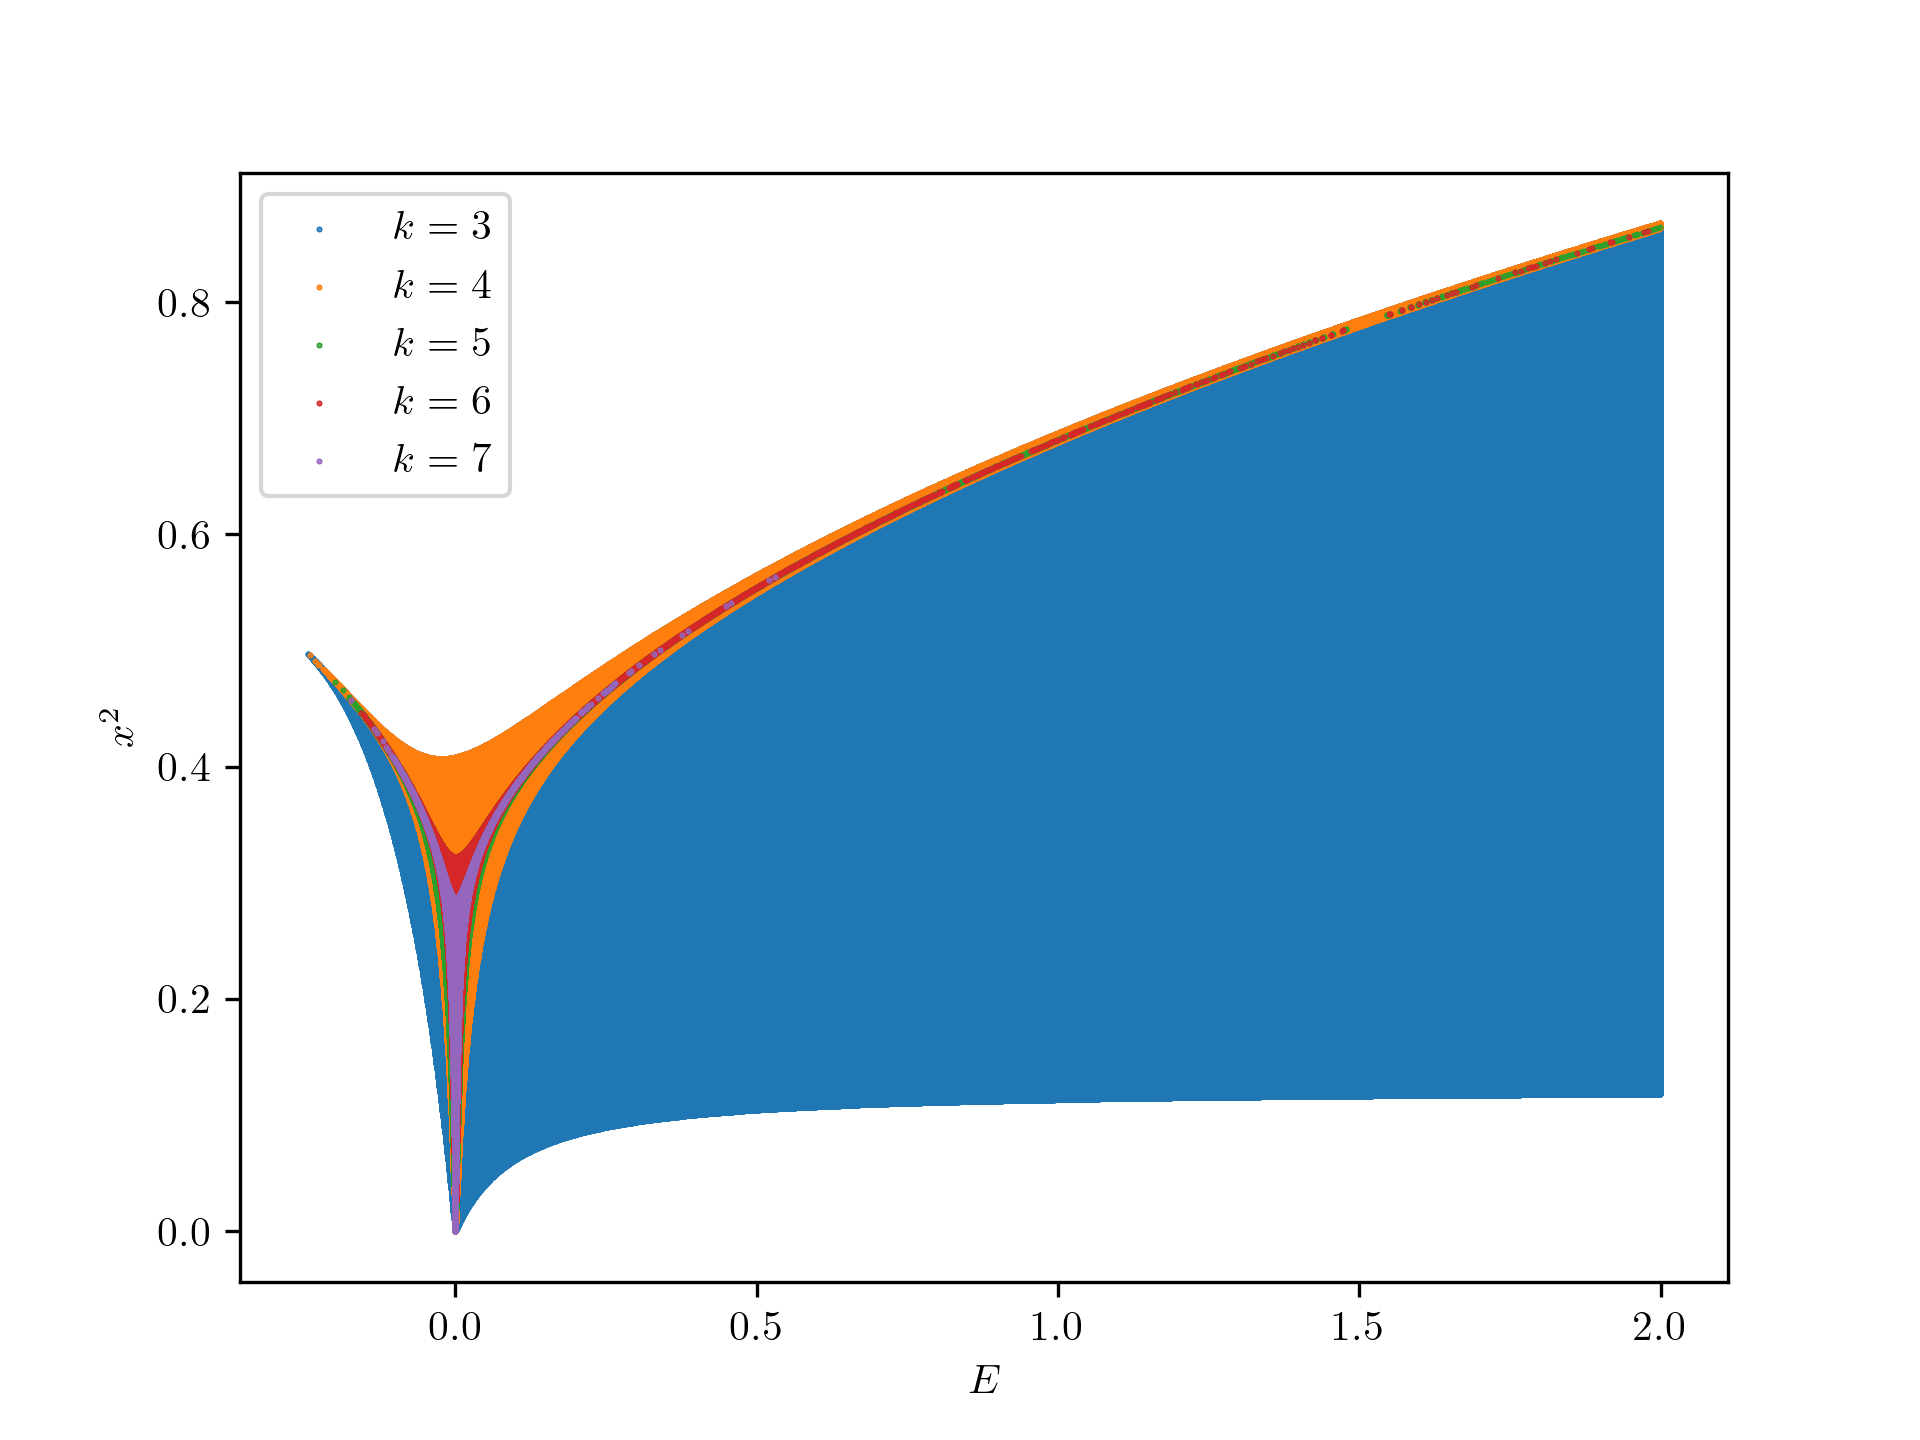
\includegraphics[width=0.8\linewidth]{double_well_xp.png}
	\caption{Allowed region in $xp$ bootstrap}
	\label{fig:doublewell}
\end{figure}
\begin{figure}
	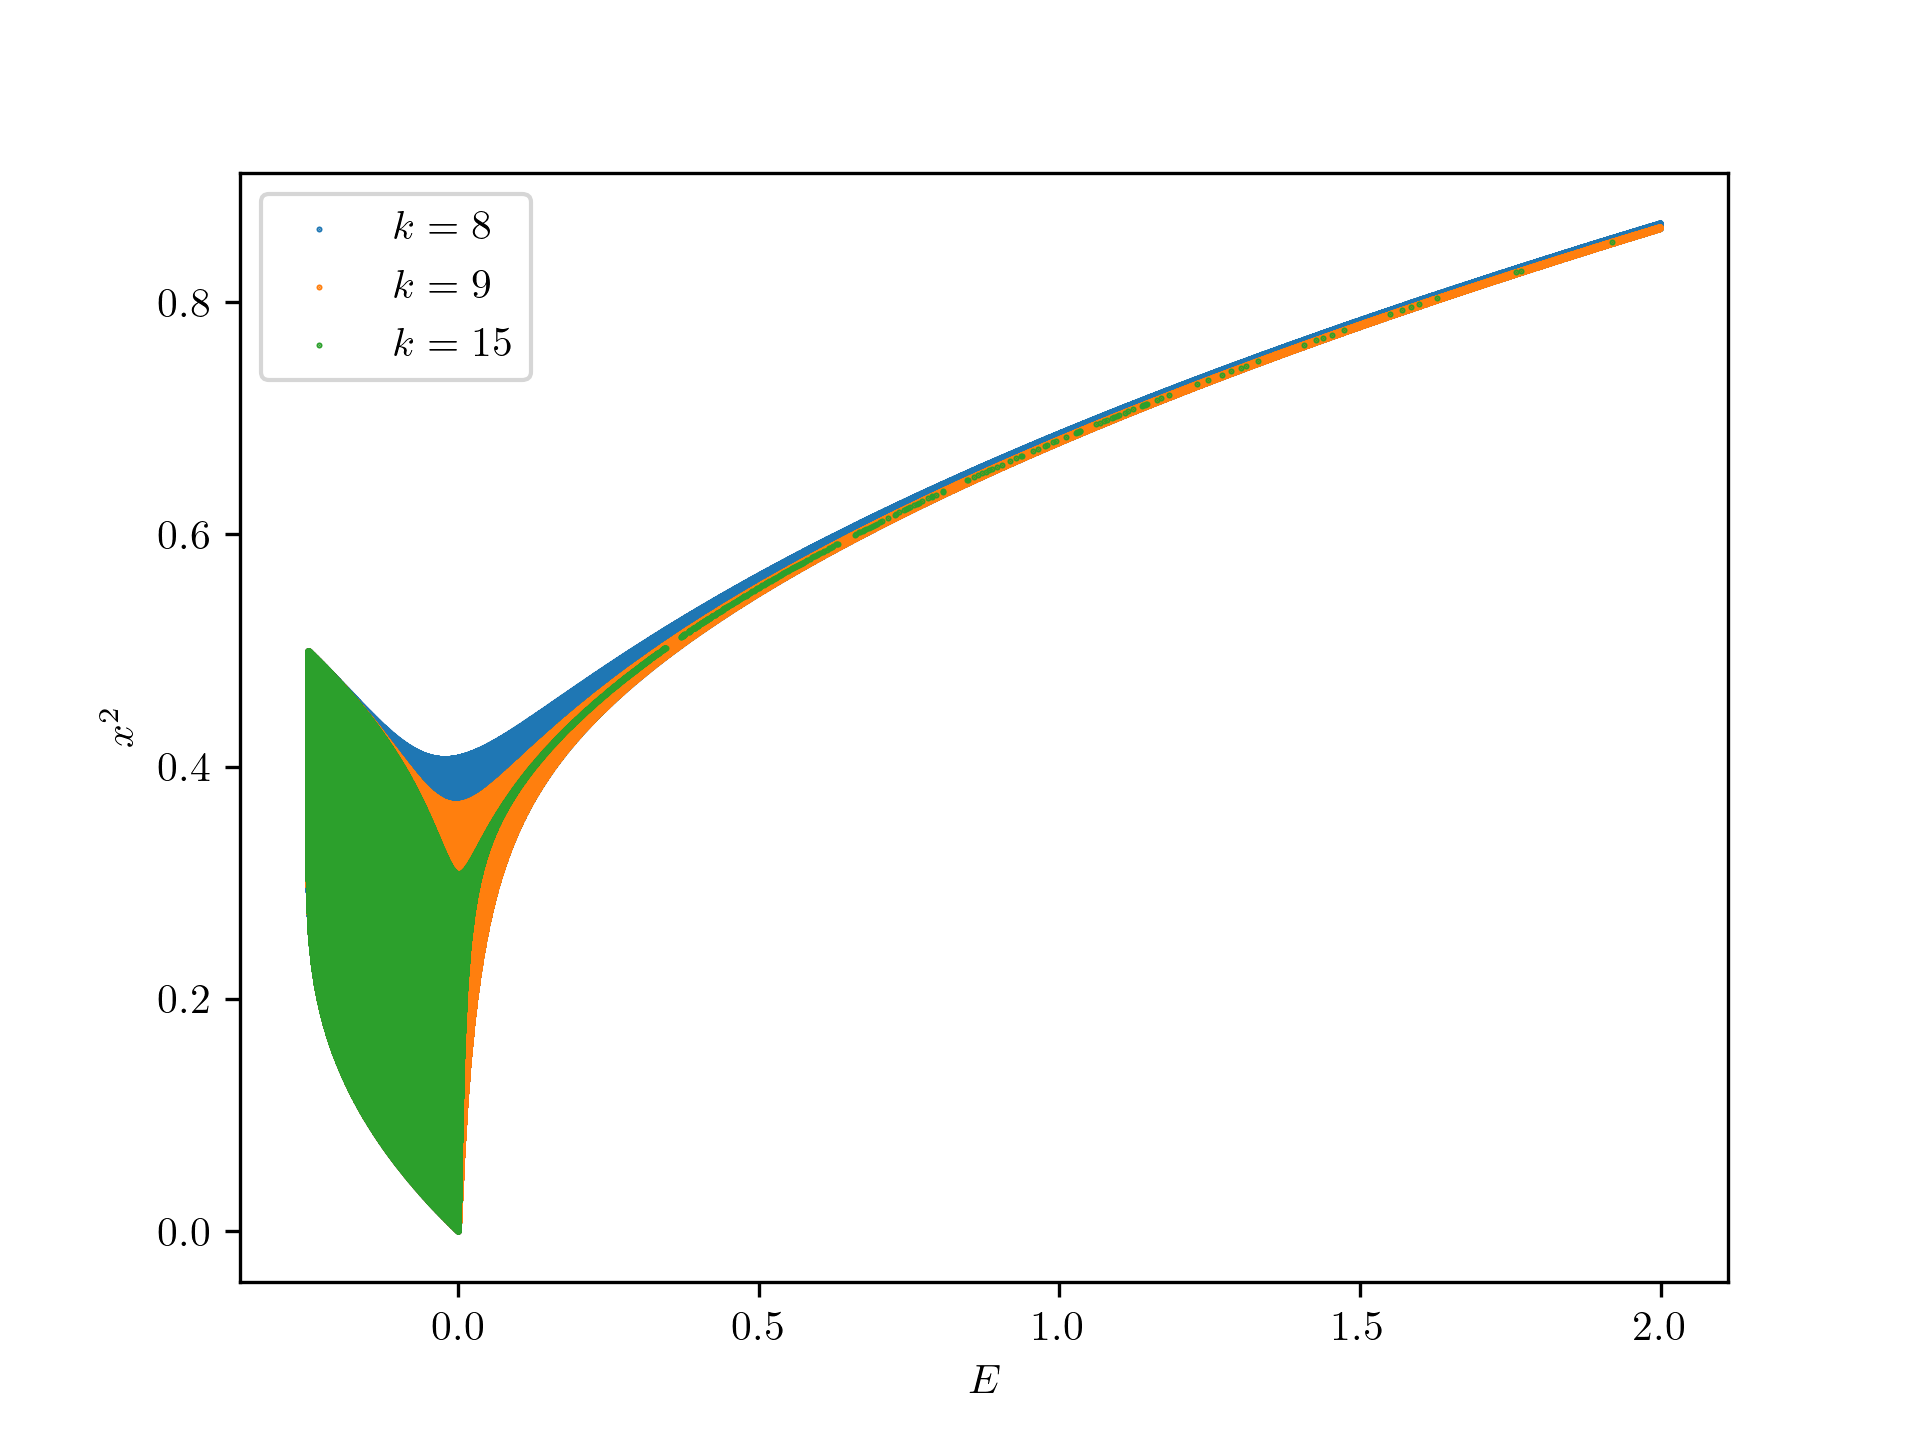
\includegraphics[width=0.8\linewidth]{double_well_x.png}
	\caption{Allowed region in $x$ bootstrap}
\end{figure}

% \begin{figure}
%     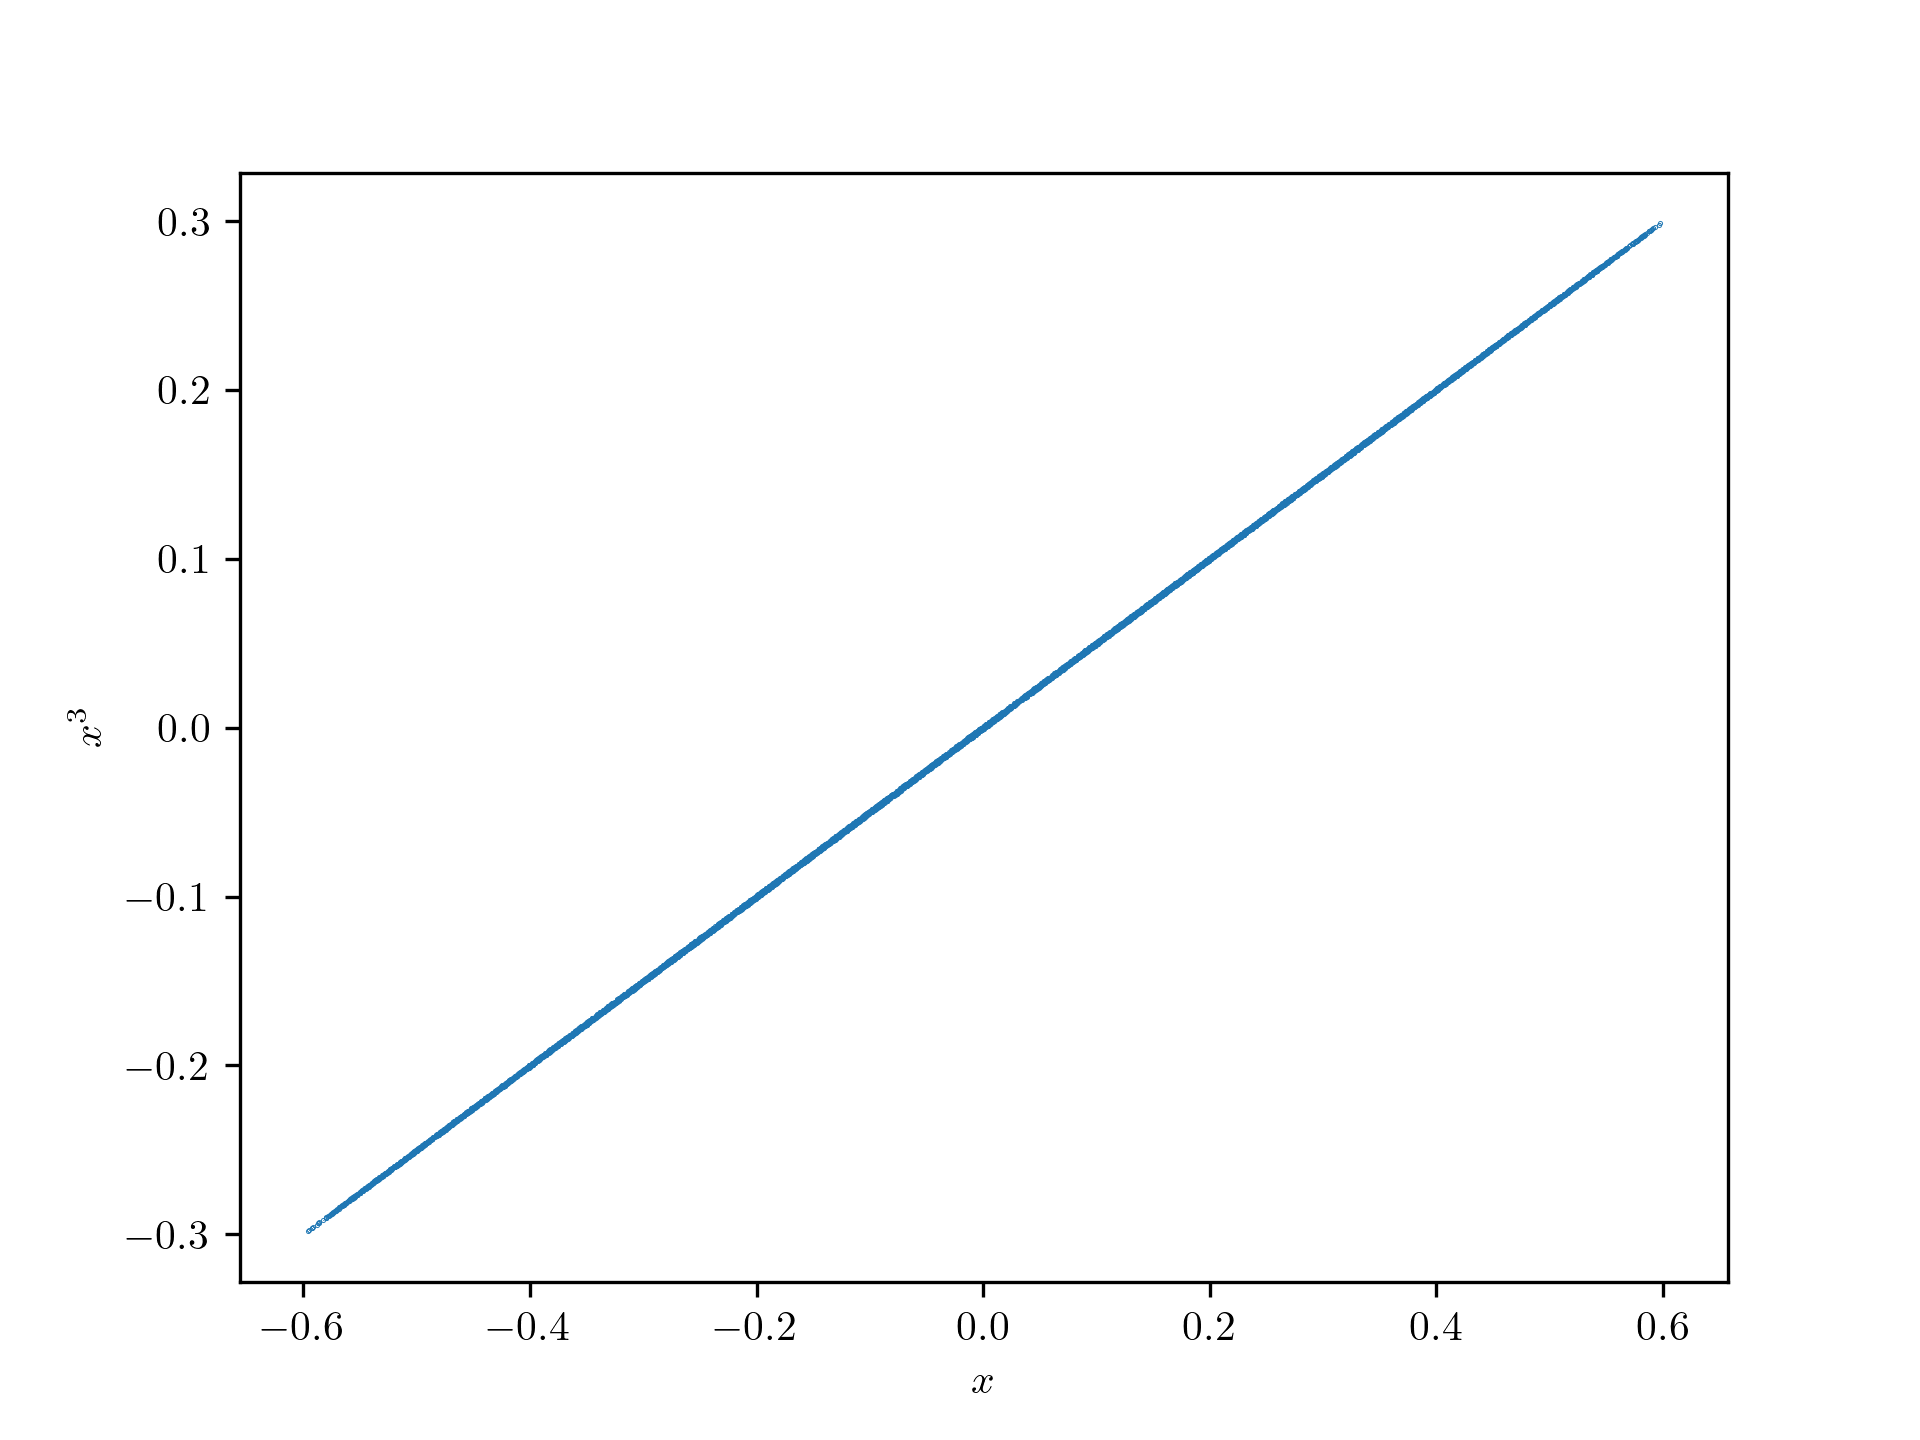
\includegraphics[width=0.8\linewidth]{13.png}
%     \caption{$\braket{x^m p^n}$ bootstrap ($k = 5$) with fixed $E = -0.1$ and $\braket{x} = 0.4052$}
%     \label{fig:xx}
% \end{figure}
%

In constrast with \cite{Nakayama_2022}, our result shows no peninsula when $E$ is negative, as we include the information of the momentum. \added{Although this $xp$ bootstrap performs poorly when $k=3$, the allowed region narrows down rapidly when $k = 4$ and it continues to shrink as $k$ gets larger.}Note that in our program the scale of the bootstrap matrix is $k^4$, which is much larger compared to the single observable bootstrap program with the scale of $k^2$. So in the case $k=5$ the size of our bootstrap matrix is $625$, about seven times bigger than that of the $x$ bootstrap. But the allowed region still doesn't shrink even when we set $k = 25$ for the $x$ only bootstrap program, so we conclude that this bootstrap in phase space does have a much stronger constraint than the single observable one.

%Like Nakayama has mentioned, $\braket{x}$ doesn't have to be zero in classical mechanics, but this method does produce a narrow region upon the assumption \eqref{eq:recur3}. So we then study the $\braket{x}$ and $\braket{x^3}$ with fixed $E$ and $\braket{x^2}$ using the $\braket{x^m p^n}$ bootstrap program, which, still turns out to be a line in Fig.~\ref{fig:xx}.

\subsection{Harmonic Oscillator and Coulomb Potential}

Consider a harmonic oscillator, its Hamiltonian is
\begin{equation}
	H = p^2 + x^2
\end{equation}
and again, we can obtain the recursion formula
\begin{align}
	2n\braket{x^{m + 1} p^{n - 1}} = 2Em\braket{x^{m - 1} p^{n - 1}} - 2m\braket{x^{m + 1} p^{n - 1}}\notag \\
	E\braket{x^m p^n} = \braket{x^m p^{n + 2}} + \braket{x^{m + 2} p^n}
\end{align}
since $\braket{x^0 p^0} = 1$ and $\braket{x} = 0$, and \eqref{eq:recur2} also holds true, we only need the initial energy $E$ to bootstrap. The result of bootstrap is shown in Fig.\ref{fig:harmonics}, as we sample $E$ from negative to positive, we can see that the negative energies are rejected by the bootstrap program. \deleted{While the $x$ only bootstrap can also generate the same plot, our approach reachs an accuracy about 100 times higher than the $x$ only bootstrap, because to obtain the same result, our method requires sampling more than 100 times as many data points as the original one.}
\begin{figure}
	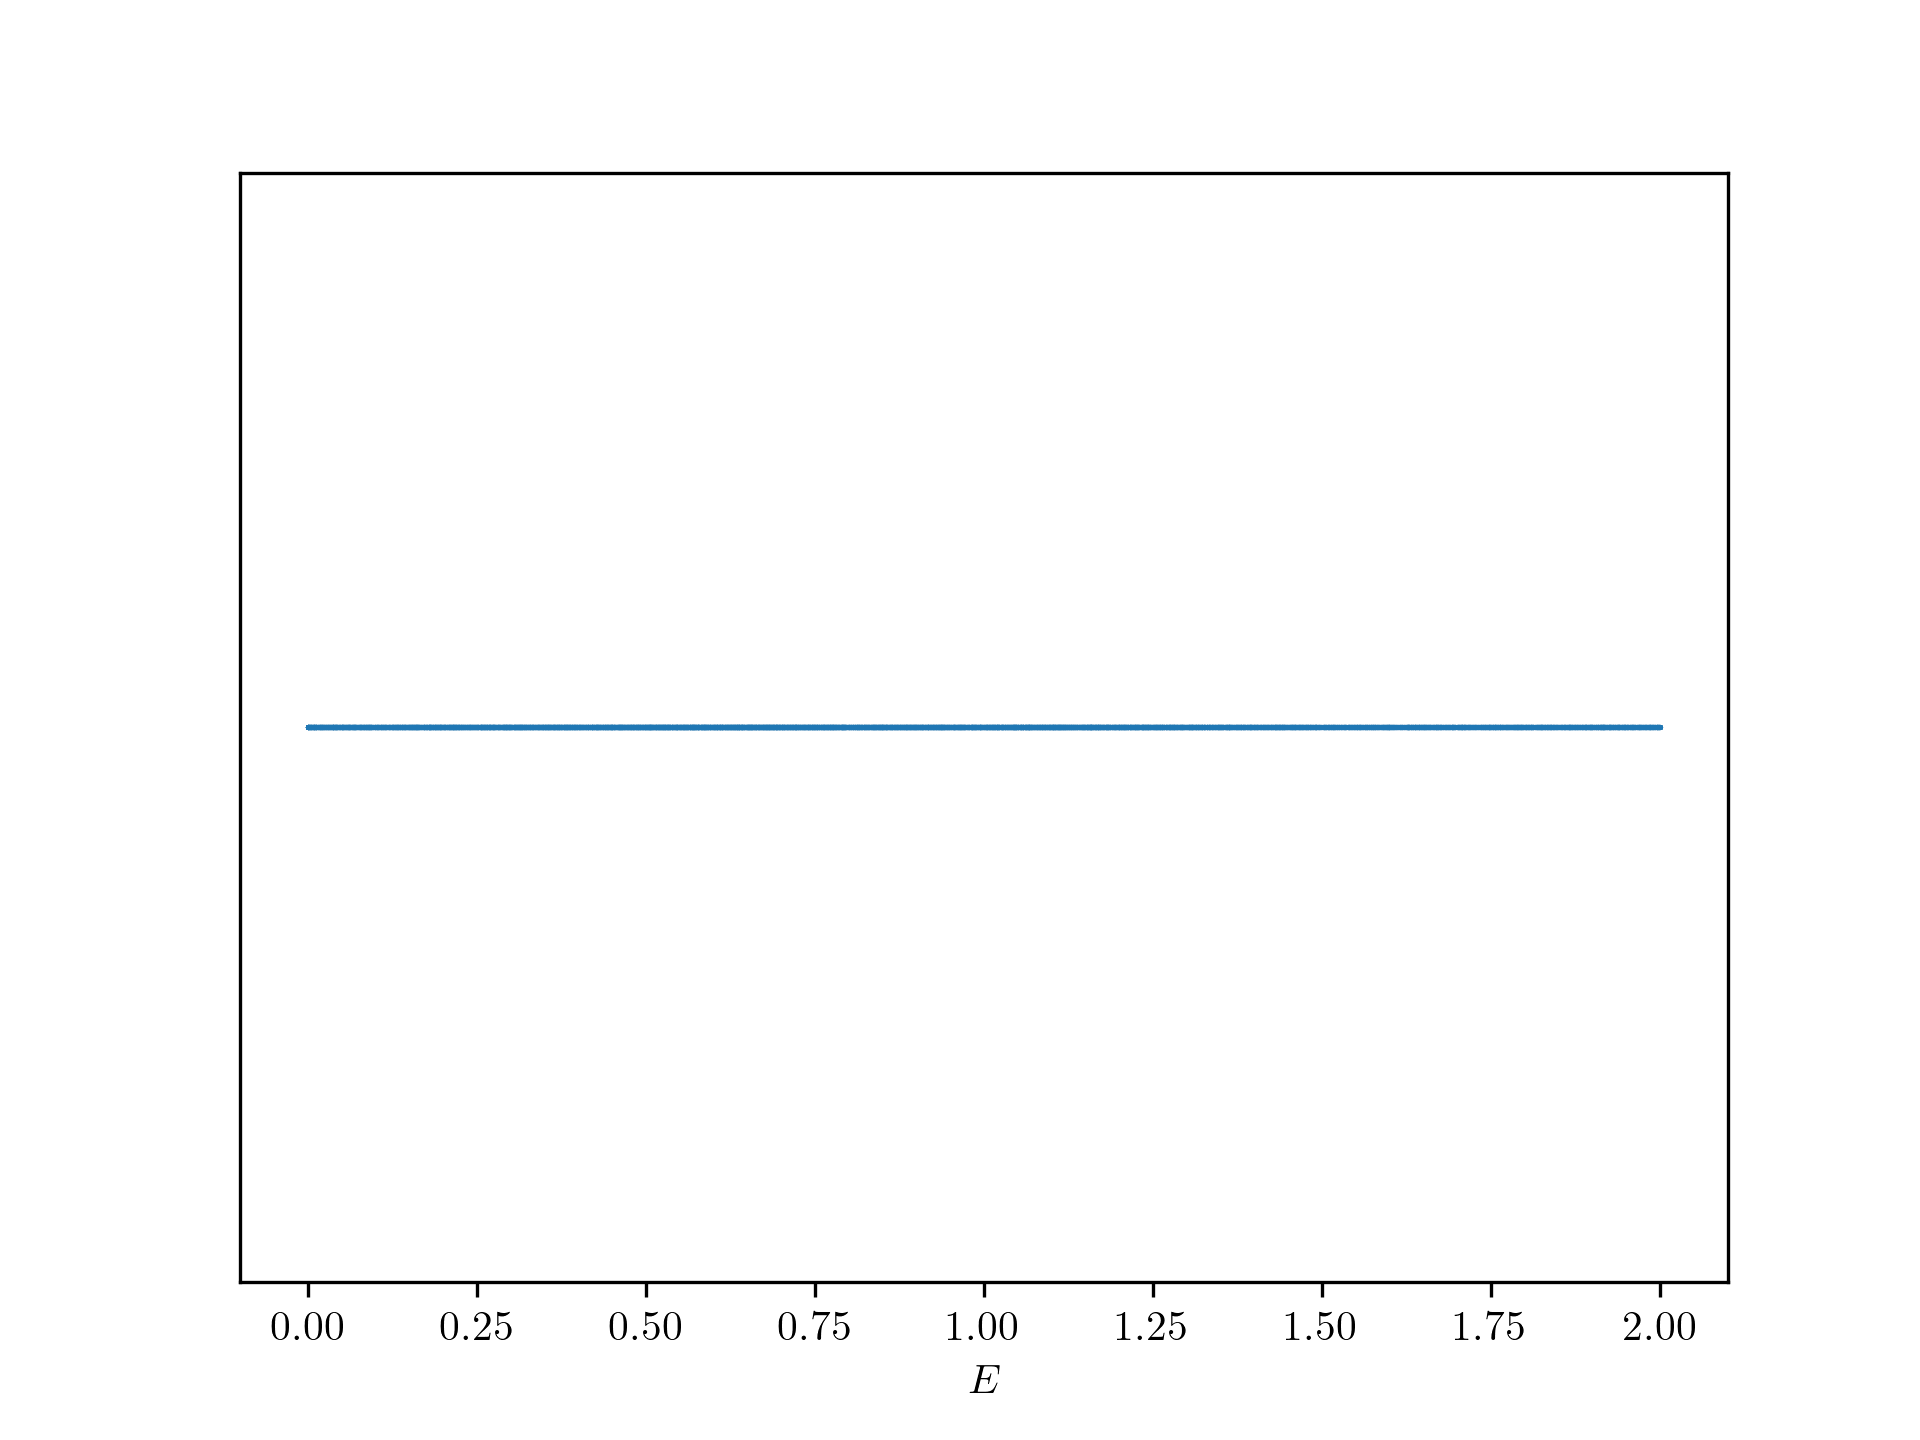
\includegraphics[width=0.8\linewidth]{harmonics.png}
	\caption{\added{Allowed regions in} \replaced{$xp$}{$\braket{x^m p^n}$} bootstrap ($k = 4$) for harmonic oscillator}
	\label{fig:harmonics}
\end{figure}

As for the coulomb potential, assume the Hamiltonian
\begin{equation}
	H = p^2 - \frac1r + \frac1{r^2}
\end{equation}
here $- \frac1r + \frac1{r^2}$ is the effective potential. The recursion equations are
\begin{align}
	2mE\braket{r^{m - 1} p^{n - 1}} = 2(m - n)\braket{r^{m - 3} p^{n - 1}} + (n - 2m)\braket{r^{m - 2} p^{n - 1}} \notag \\
	E\braket{r^m p^n} = \braket{r^m p^{n + 2}} - \braket{r^{m - 1} p^n} + \braket{r^{m - 2} p^n} \label{eq:coul}
\end{align}
Substituting $m = n = 1$ into the first equation we can get
\begin{equation}
	2E = -\braket{r^{-1}}
\end{equation}
which is the Virial theorem. \replaced{This time we only need $E$ in the $x$ bootstrap and the result is shown in Fig.\ref{fig:coulomb0}. But for the $xp$ bootstrap we also need the $\braket{r^{-2}}$ because at some points the coefficients in \eqref{eq:coul} turn to 0 and thus breaking the recursion. The initial value $\braket{r^{-2}}$ gives the exact information we need to patch up these points, together with equation \eqref{eq:recur2} the result of bootstrap is shown in Fig\ref{fig:coulomb1}. We can see that our $xp$ bootstrap excludes the positive $E$ which will cause the $r$ go negative, but the nuisance here is that we need to pay extra attention to the numerical precision, for more details see the Appendix.} {With the equation \eqref{eq:recur2}, again we only need $E$ to bootstrap the coulomb potential. The result is shown in Fig\ref{fig:coulomb0}. However, this time we failed to find any points using $x^m p^n$ bootstrap, we speculate that this is due to insufficient numerical precision. But the $x^m$ bootstrap is doing great, at least we successfully find the allowed energy.}
\begin{figure}
	\centering
	\begin{minipage}{0.45\textwidth}
		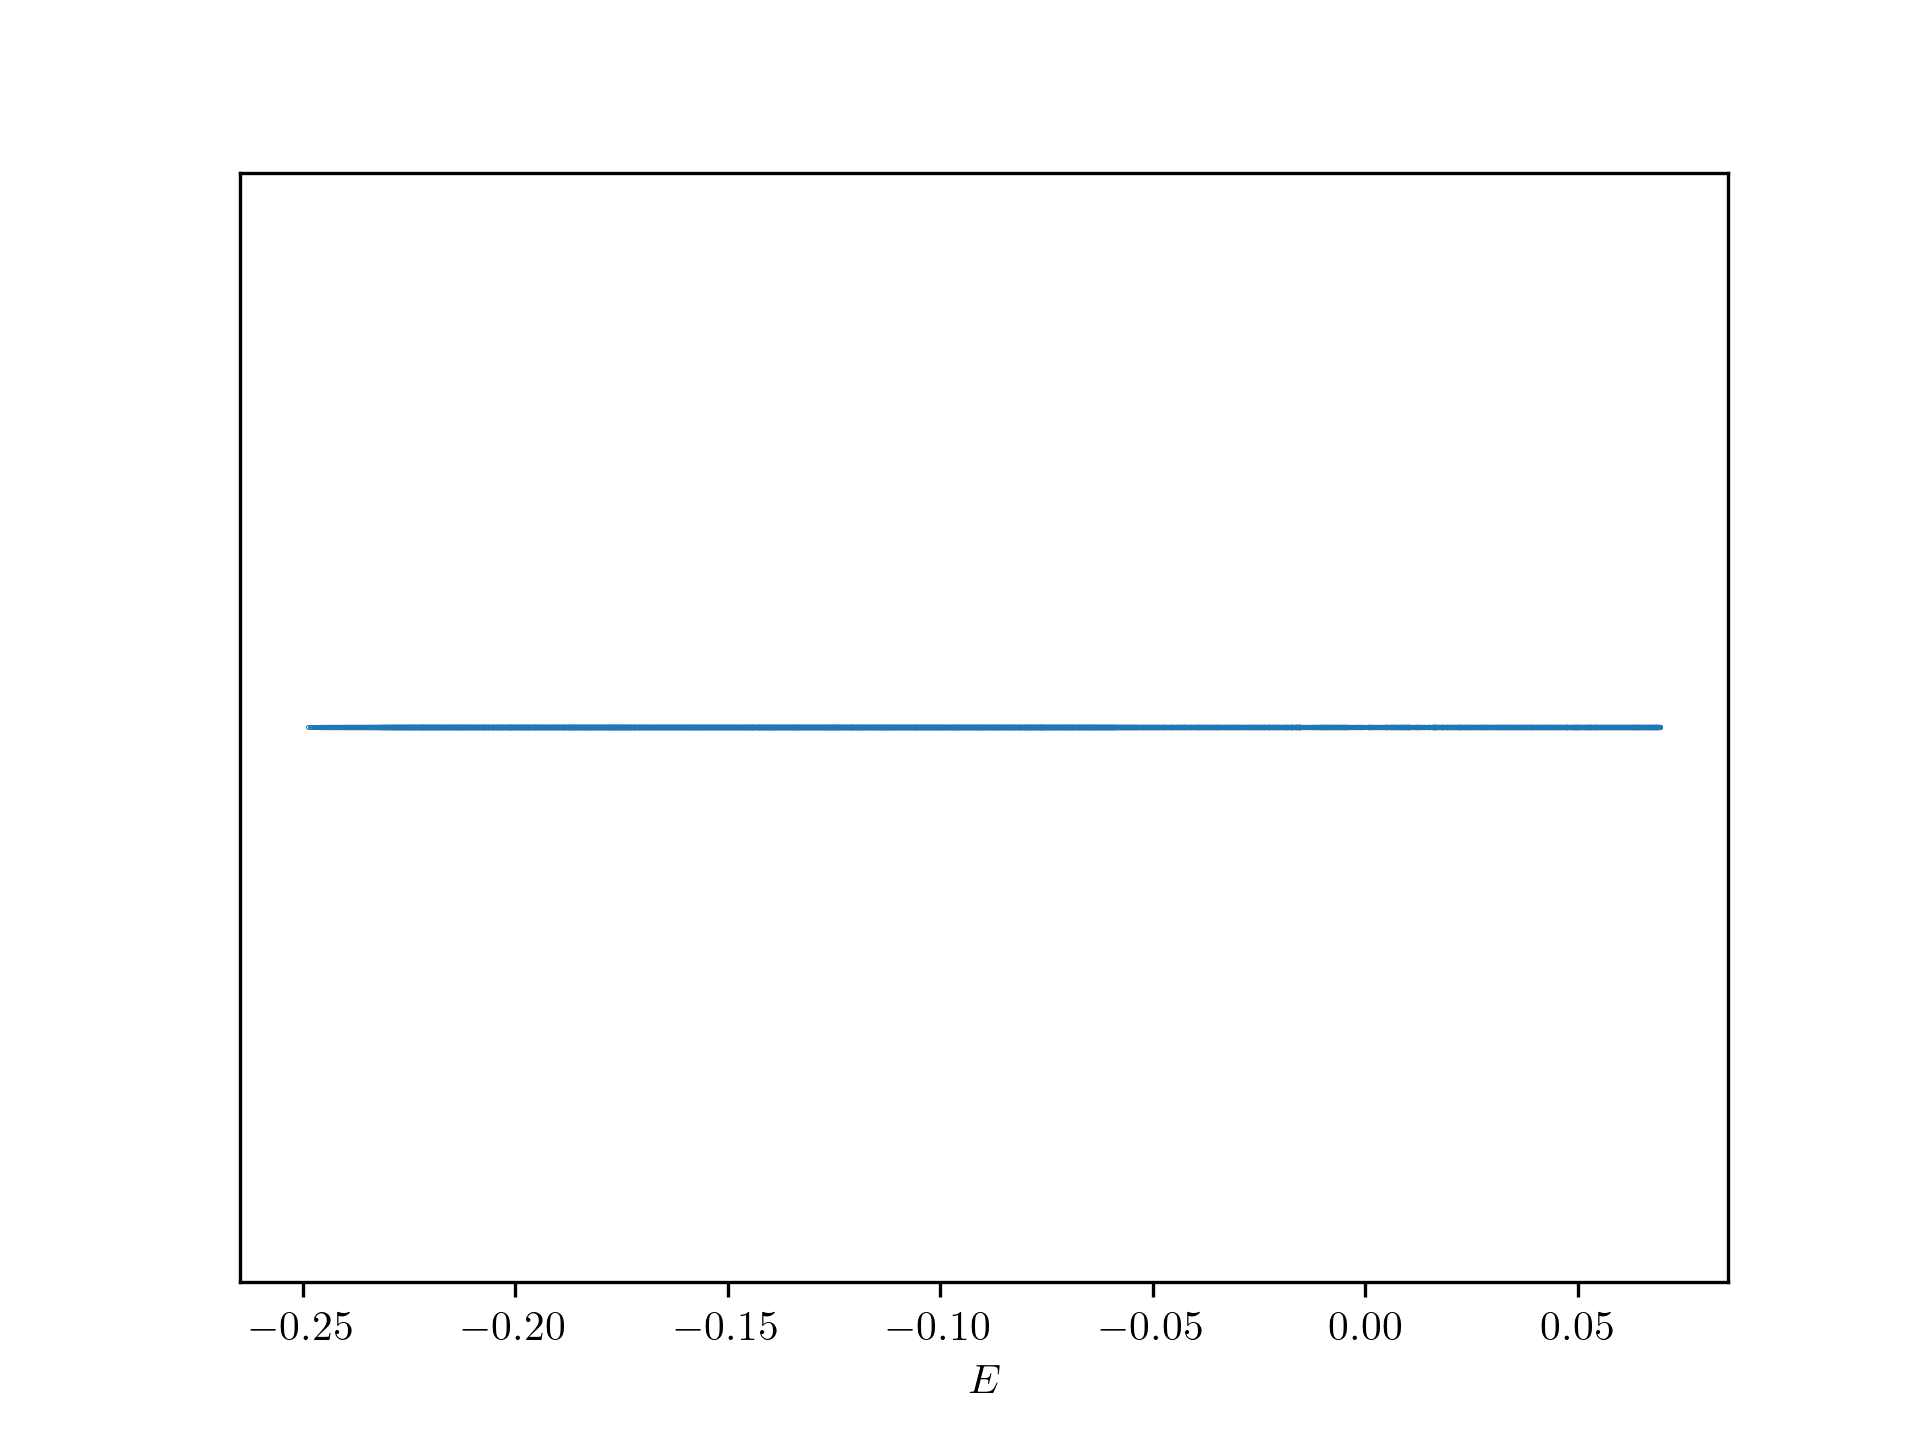
\includegraphics[width=\linewidth]{coulomb.png}
		\caption{\added{Allowed regions in $x$} \deleted{$\braket{x^m}$} bootstrap ($k = 8$) for coulomb potential}
		\label{fig:coulomb0}
	\end{minipage}
	\hfill
	\begin{minipage}{0.45\textwidth}
		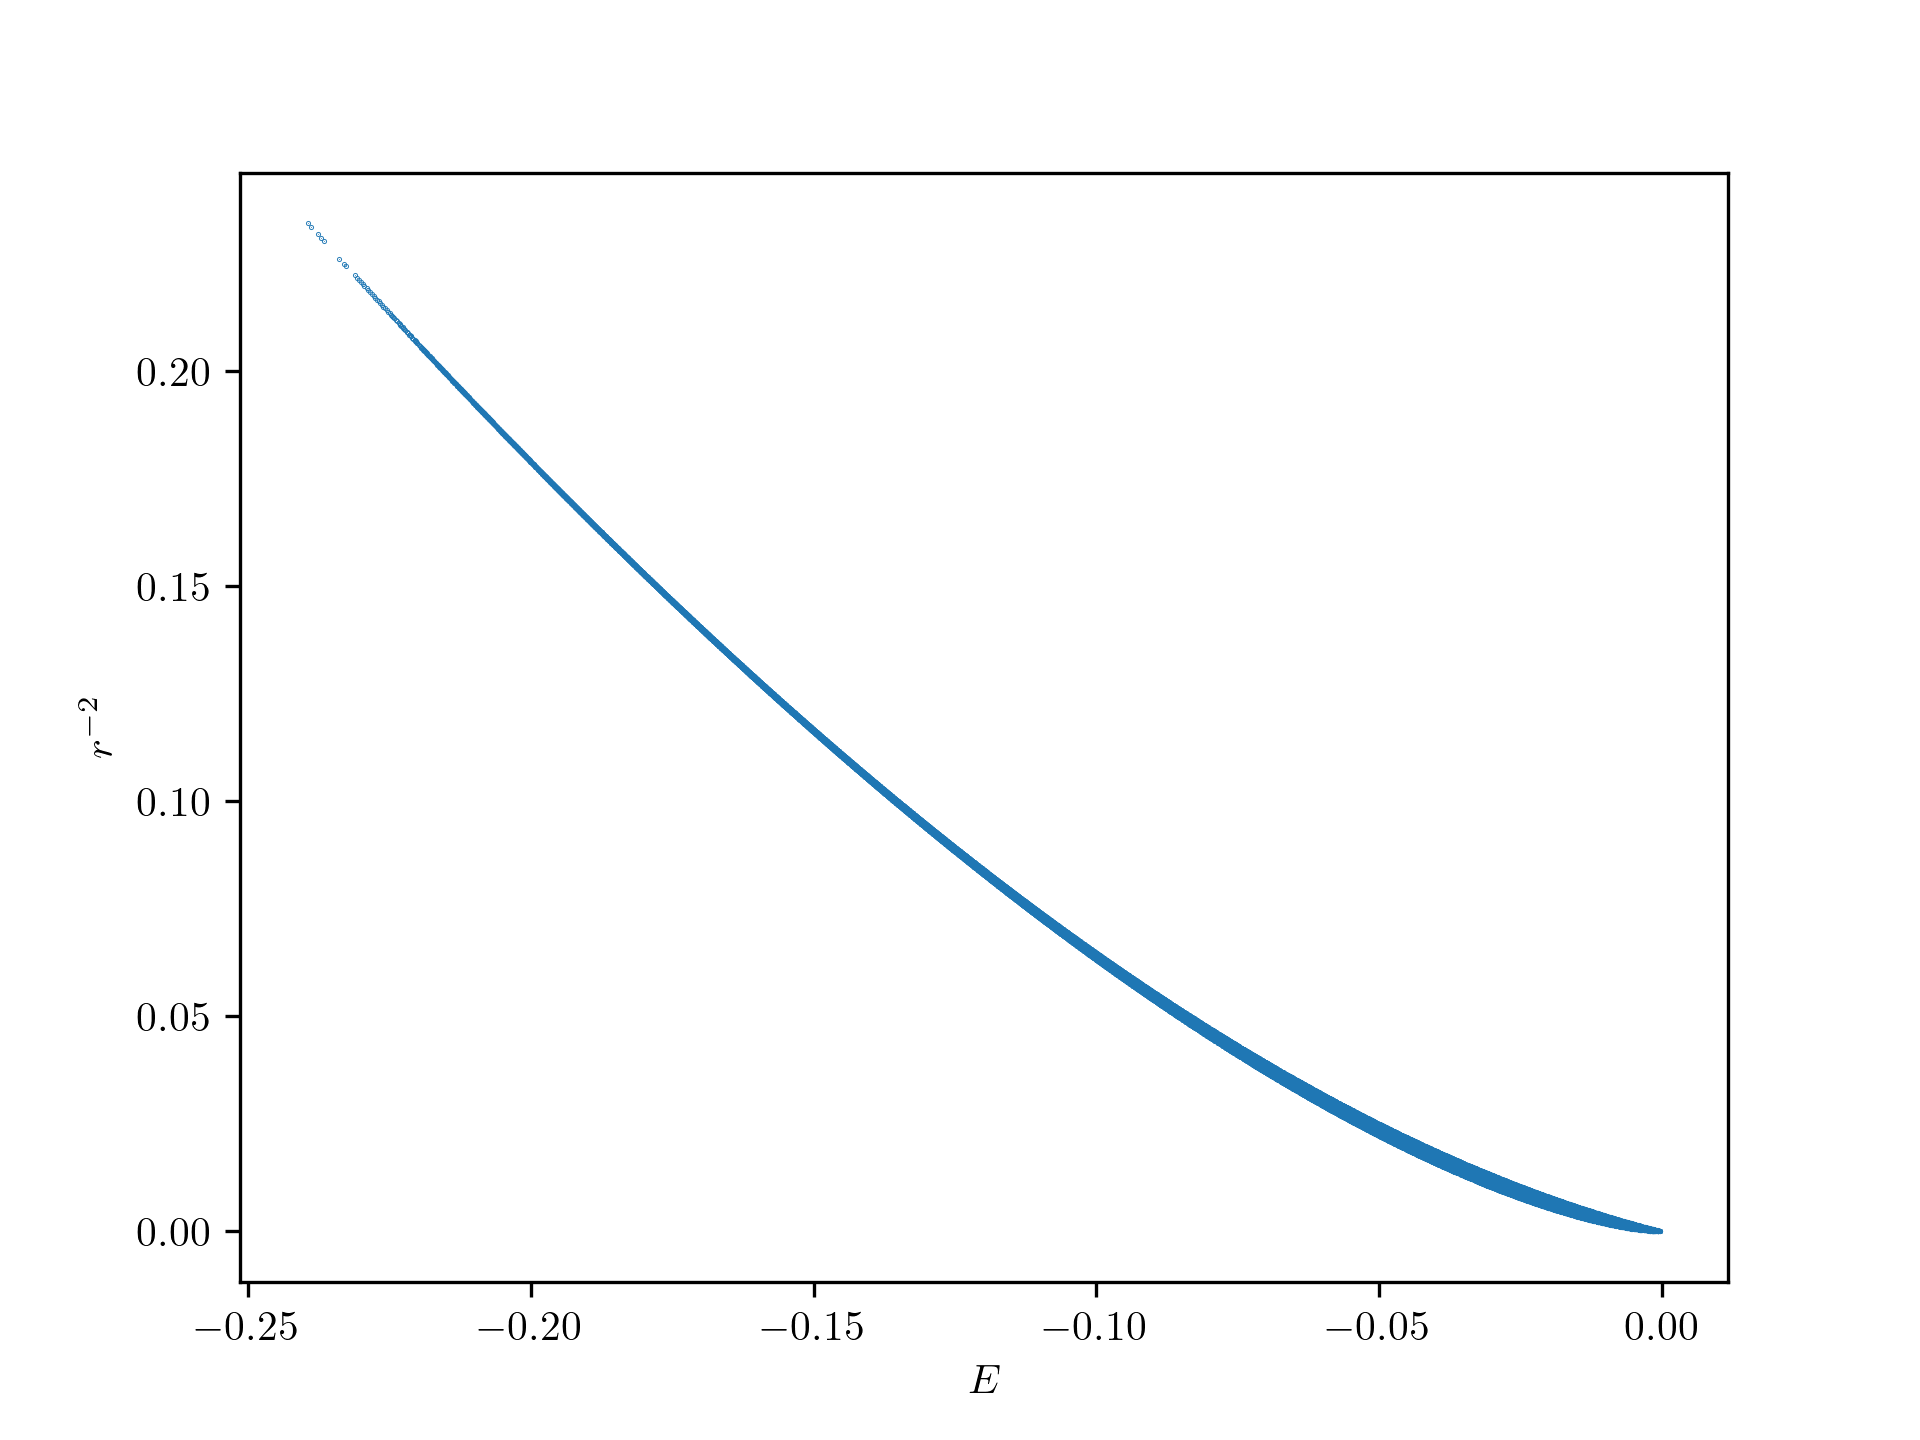
\includegraphics[width=\linewidth]{coulomb_double.png}
		\caption{Allowed regions in $xp$ bootstrap ($k = 3$) for coulomb potential}
		\label{fig:coulomb1}
	\end{minipage}

\end{figure}

\subsection{Non-Relativistic TODA model}
For a non-relativistic TODA model, the Hamiltonian might be written as
\begin{equation}
	H = p^2 + e^x + e^{-x}
\end{equation}
the recursion equations are
\begin{align}
	(n + 2m)\braket{e^{m + 1} p^{n - 1}} = 2E\braket{e^m p^{n - 1}} + (n - 2m)\braket{e^{m - 1} p^{n - 1}}\notag \\
	E\braket{e^{mx} p^n} = \braket{e^{mx} p^{n + 2}} + \braket{e^{(m + 1)x} p^n} + \braket{e^{(m - 1)x} p^n}
\end{align}
and studying $\braket{\{H, e^{mx}\}}$ we have
\begin{equation}
	\braket{e^{(m - 1)x} p} = 0
\end{equation}
using the initial parameters $E$ and $\braket{e^x}$, the bootstrap result is shown in Fig.\ref{fig:toda}
\begin{figure}
	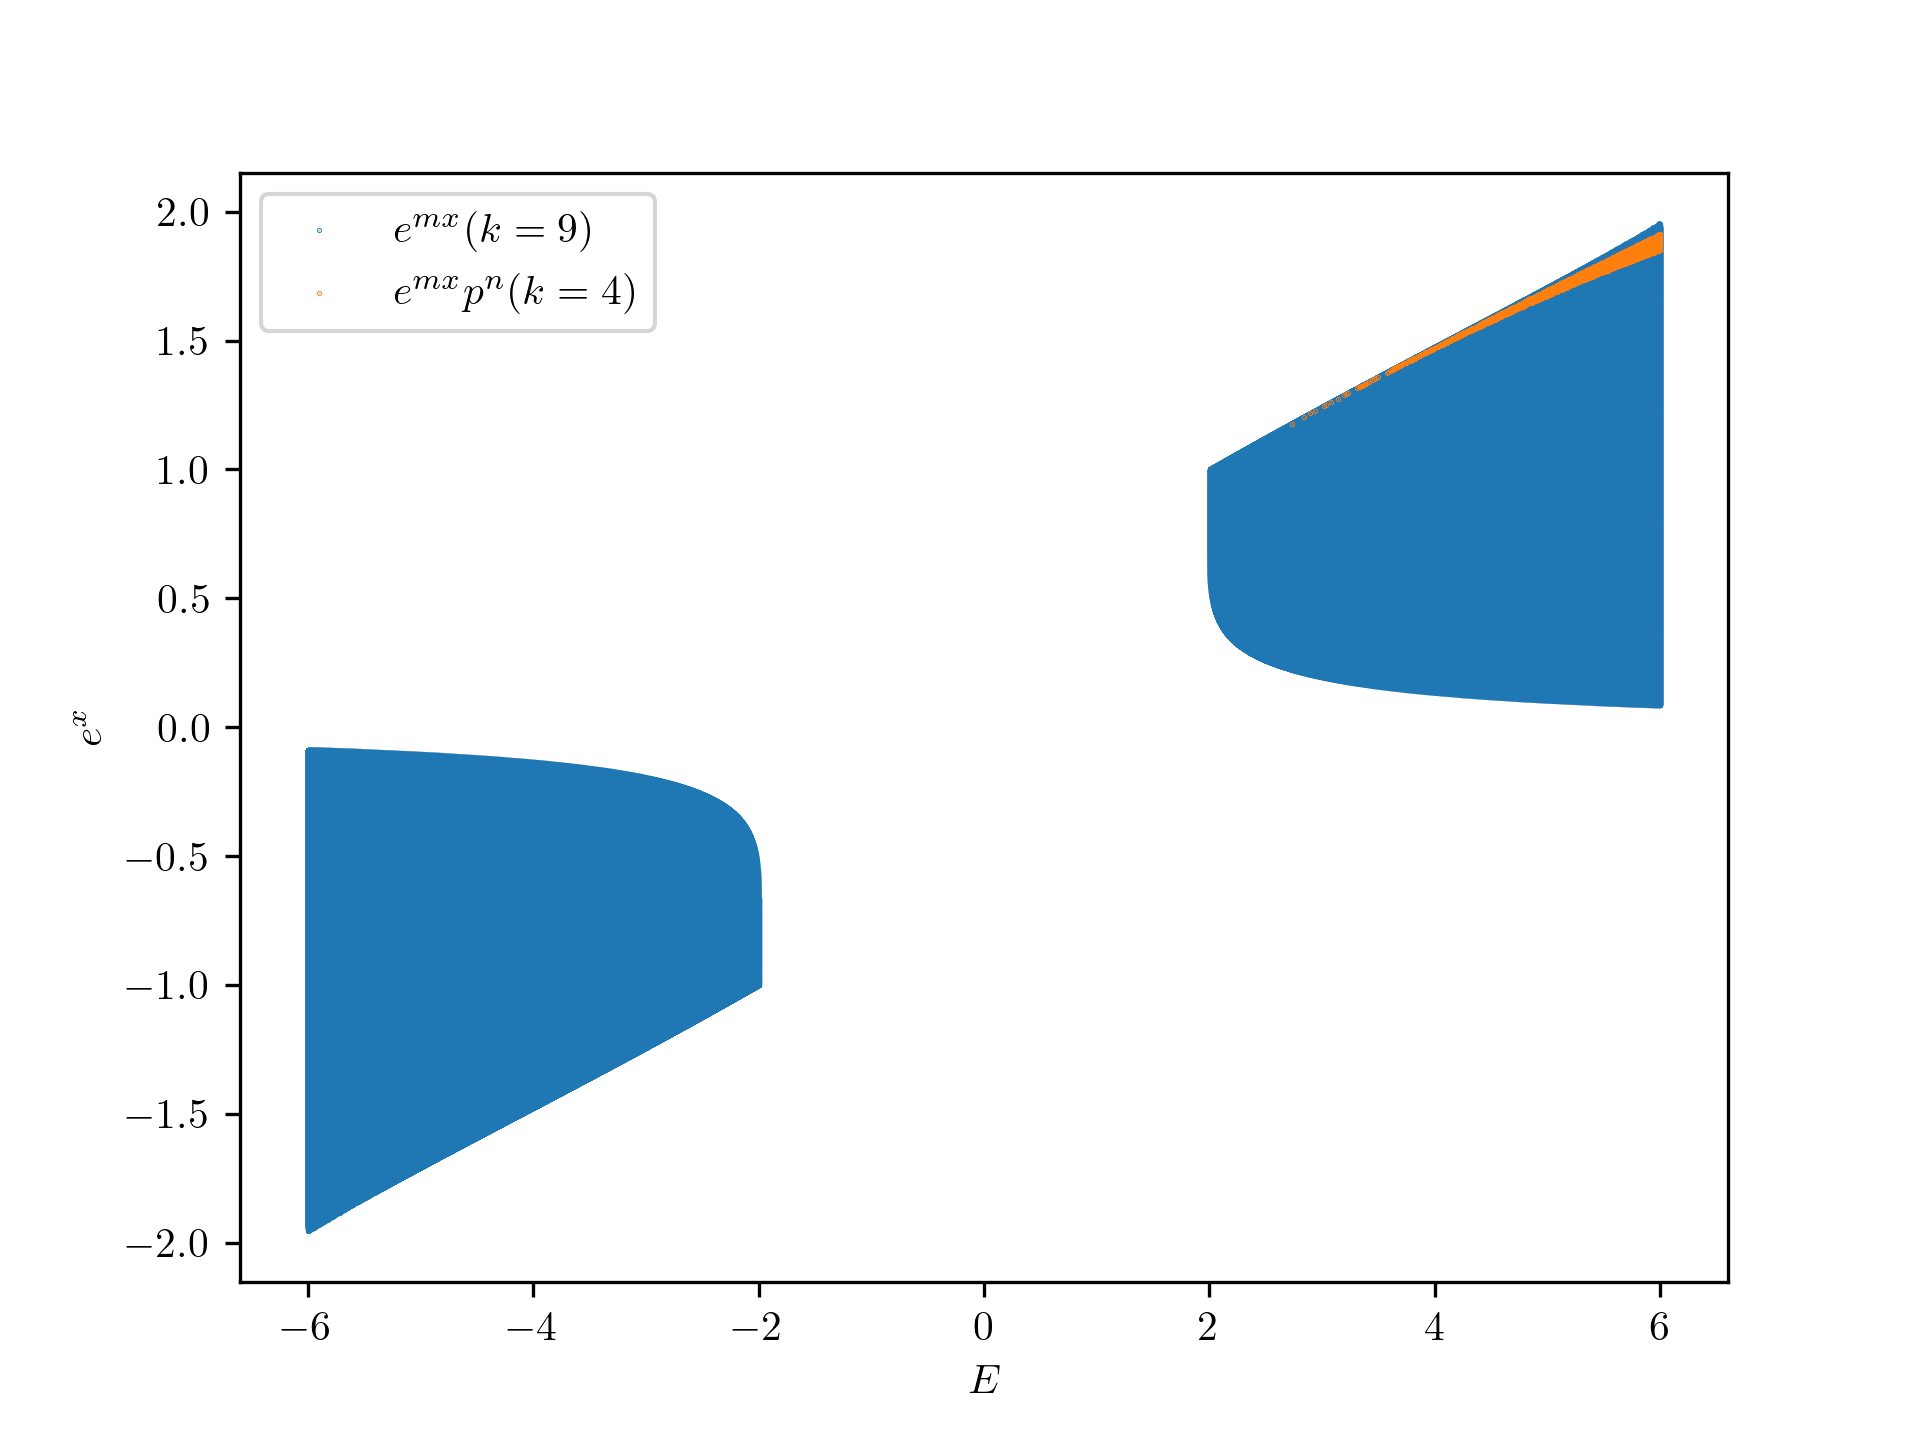
\includegraphics[width=0.8\linewidth]{toda_compare.png}
	\caption{\added{Allowed regions in $xp$} bootstrap for non-relativistic TODA model}
	\label{fig:toda}
\end{figure}

The two observables bootstrap shows a much stronger constraint than the single one, in this non-relativistic TODA mode the $e^{mx}$ bootstrap even fails to reject the negative $E$, and results in a much larger region. Our approach may have better precision, yet the allowed region still tends to diverge when $E$ goes large in Fig.~\ref{fig:todal}.

\begin{figure}
	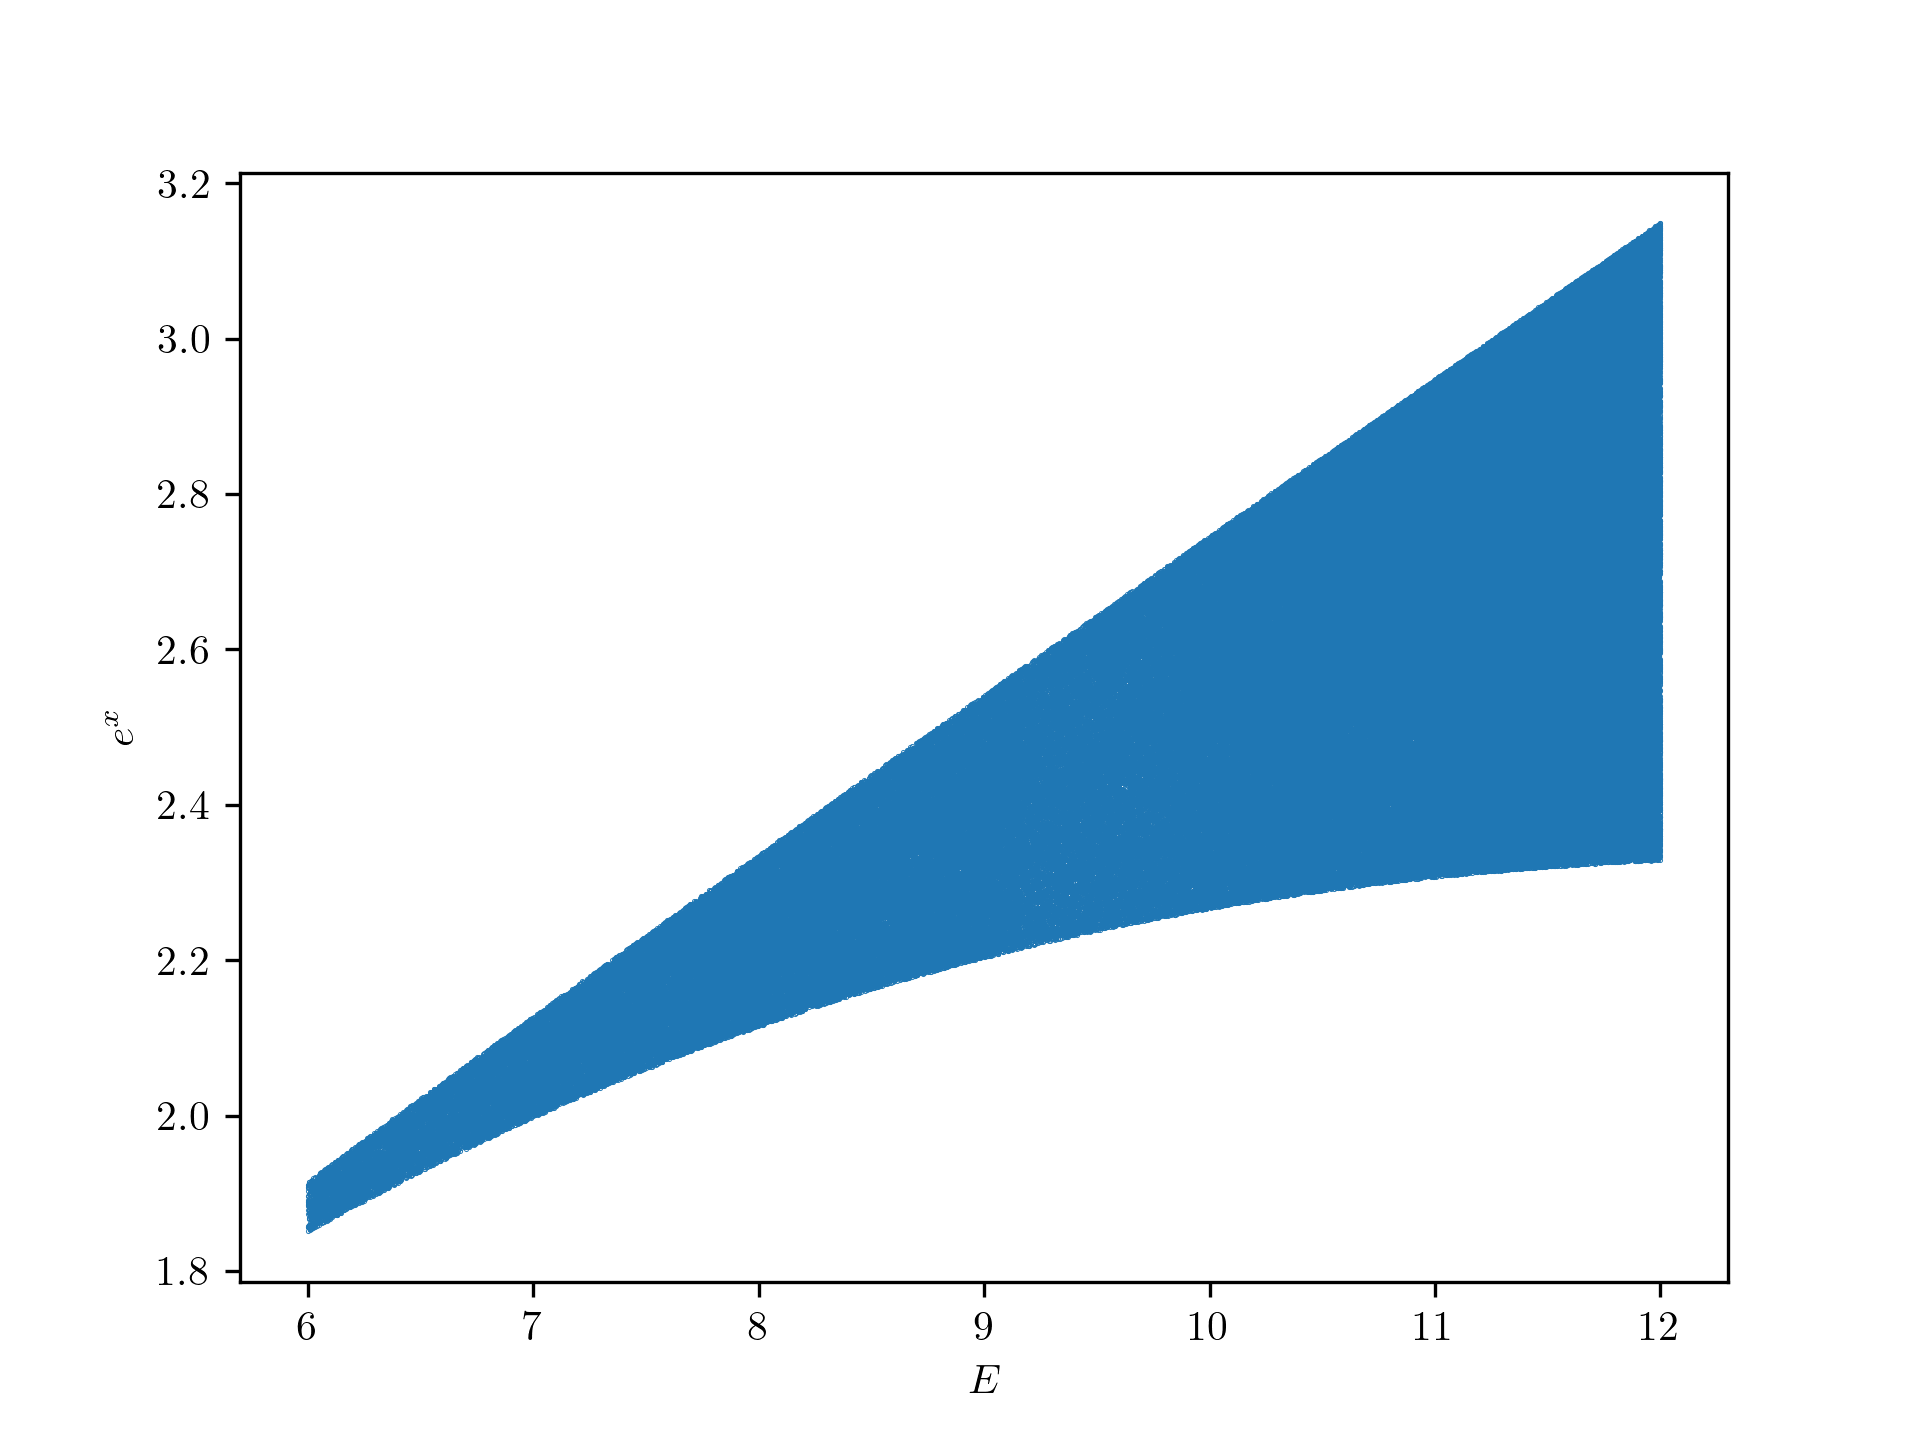
\includegraphics[width=0.8\linewidth]{todal.png}
	\caption{Allowed region diverges as $E$ grows}
	\label{fig:todal}
\end{figure}

\section{Conclusions}
In this paper, we study two different bootstrap approaches in various models, our approach outperforms the single observable bootstrap program in most cases.\deleted{in some models e.g. double-well, non-relativistic TODA model, while in other two models our bootstrap in phase space fails to achieve a satisfactory result, the single observable one already restricts the model pretty well}.\added{We've seen that it cancels the sector region in double well potential, excludes some invalid $E$s in both harmonic oscillator and non-relativistic TODA model.}
Although it performs better and achieves a much higher precision, it still fails to converge to the exact solution, and even tends to diverge. Like in the situations that $E \to 0$ in the double-well potential, $E \to \infty$ in the non-relativistic TODA model, we might still be missing some information to pin point the final answer.

\section*{Acknowledgements}
I would like to thank Dong Bai for discussions and encouragements. I would also like to acknowledge Zhaobin Huang for reading the manuscript and valuable comments.


% If in two-column mode, this environment will change to single-column
% format so that long equations can be displayed. Use
% sparingly.
%\begin{widetext}
% put long equation here
%\end{widetext}

% figures should be put into the text as floats.
% Use the graphics or graphicx packages (distributed with LaTeX2e)
% and the \includegraphics macro defined in those packages.
% See the LaTeX Graphics Companion by Michel Goosens, Sebastian Rahtz,
% and Frank Mittelbach for instance.
%
% Here is an example of the general form of a figure:
% Fill in the caption in the braces of the \caption{} command. Put the label
% that you will use with \ref{} command in the braces of the \label{} command.
% Use the figure* environment if the figure should span across the
% entire page. There is no need to do explicit centering.

% \begin{figure}
% \includegraphics{}%
% \caption{\label{}}
% \end{figure}

% Surround figure environment with turnpage environment for landscape
% figure
% \begin{turnpage}
% \begin{figure}
% \includegraphics{}%
% \caption{\label{}}
% \end{figure}
% \end{turnpage}

% tables should appear as floats within the text
%
% Here is an example of the general form of a table:
% Fill in the caption in the braces of the \caption{} command. Put the label
% that you will use with \ref{} command in the braces of the \label{} command.
% Insert the column specifiers (l, r, c, d, etc.) in the empty braces of the
% \begin{tabular}{} command.
% The ruledtabular enviroment adds doubled rules to table and sets a
% reasonable default table settings.
% Use the table* environment to get a full-width table in two-column
% Add \usepackage{longtable} and the longtable (or longtable*}
% environment for nicely formatted long tables. Or use the the [H]
% placement option to break a long table (with less control than
% in longtable).
% \begin{table}%[H] add [H] placement to break table across pages
% \caption{\label{}}
% \begin{ruledtabular}
% \begin{tabular}{}
% Lines of table here ending with \\
% \end{tabular}
% \end{ruledtabular}
% \end{table}

% Surround table environment with turnpage environment for landscape
% table
% \begin{turnpage}
% \begin{table}
% \caption{\label{}}
% \begin{ruledtabular}
% \begin{tabular}{}
% \end{tabular}
% \end{ruledtabular}
% \end{table}
% \end{turnpage}

% Specify following sections are appendices. Use \appendix* if there
% only one appendix.
%\appendix
%\section{}
\appendix* 
	\section{Numerical details}
	\begin{figure}
		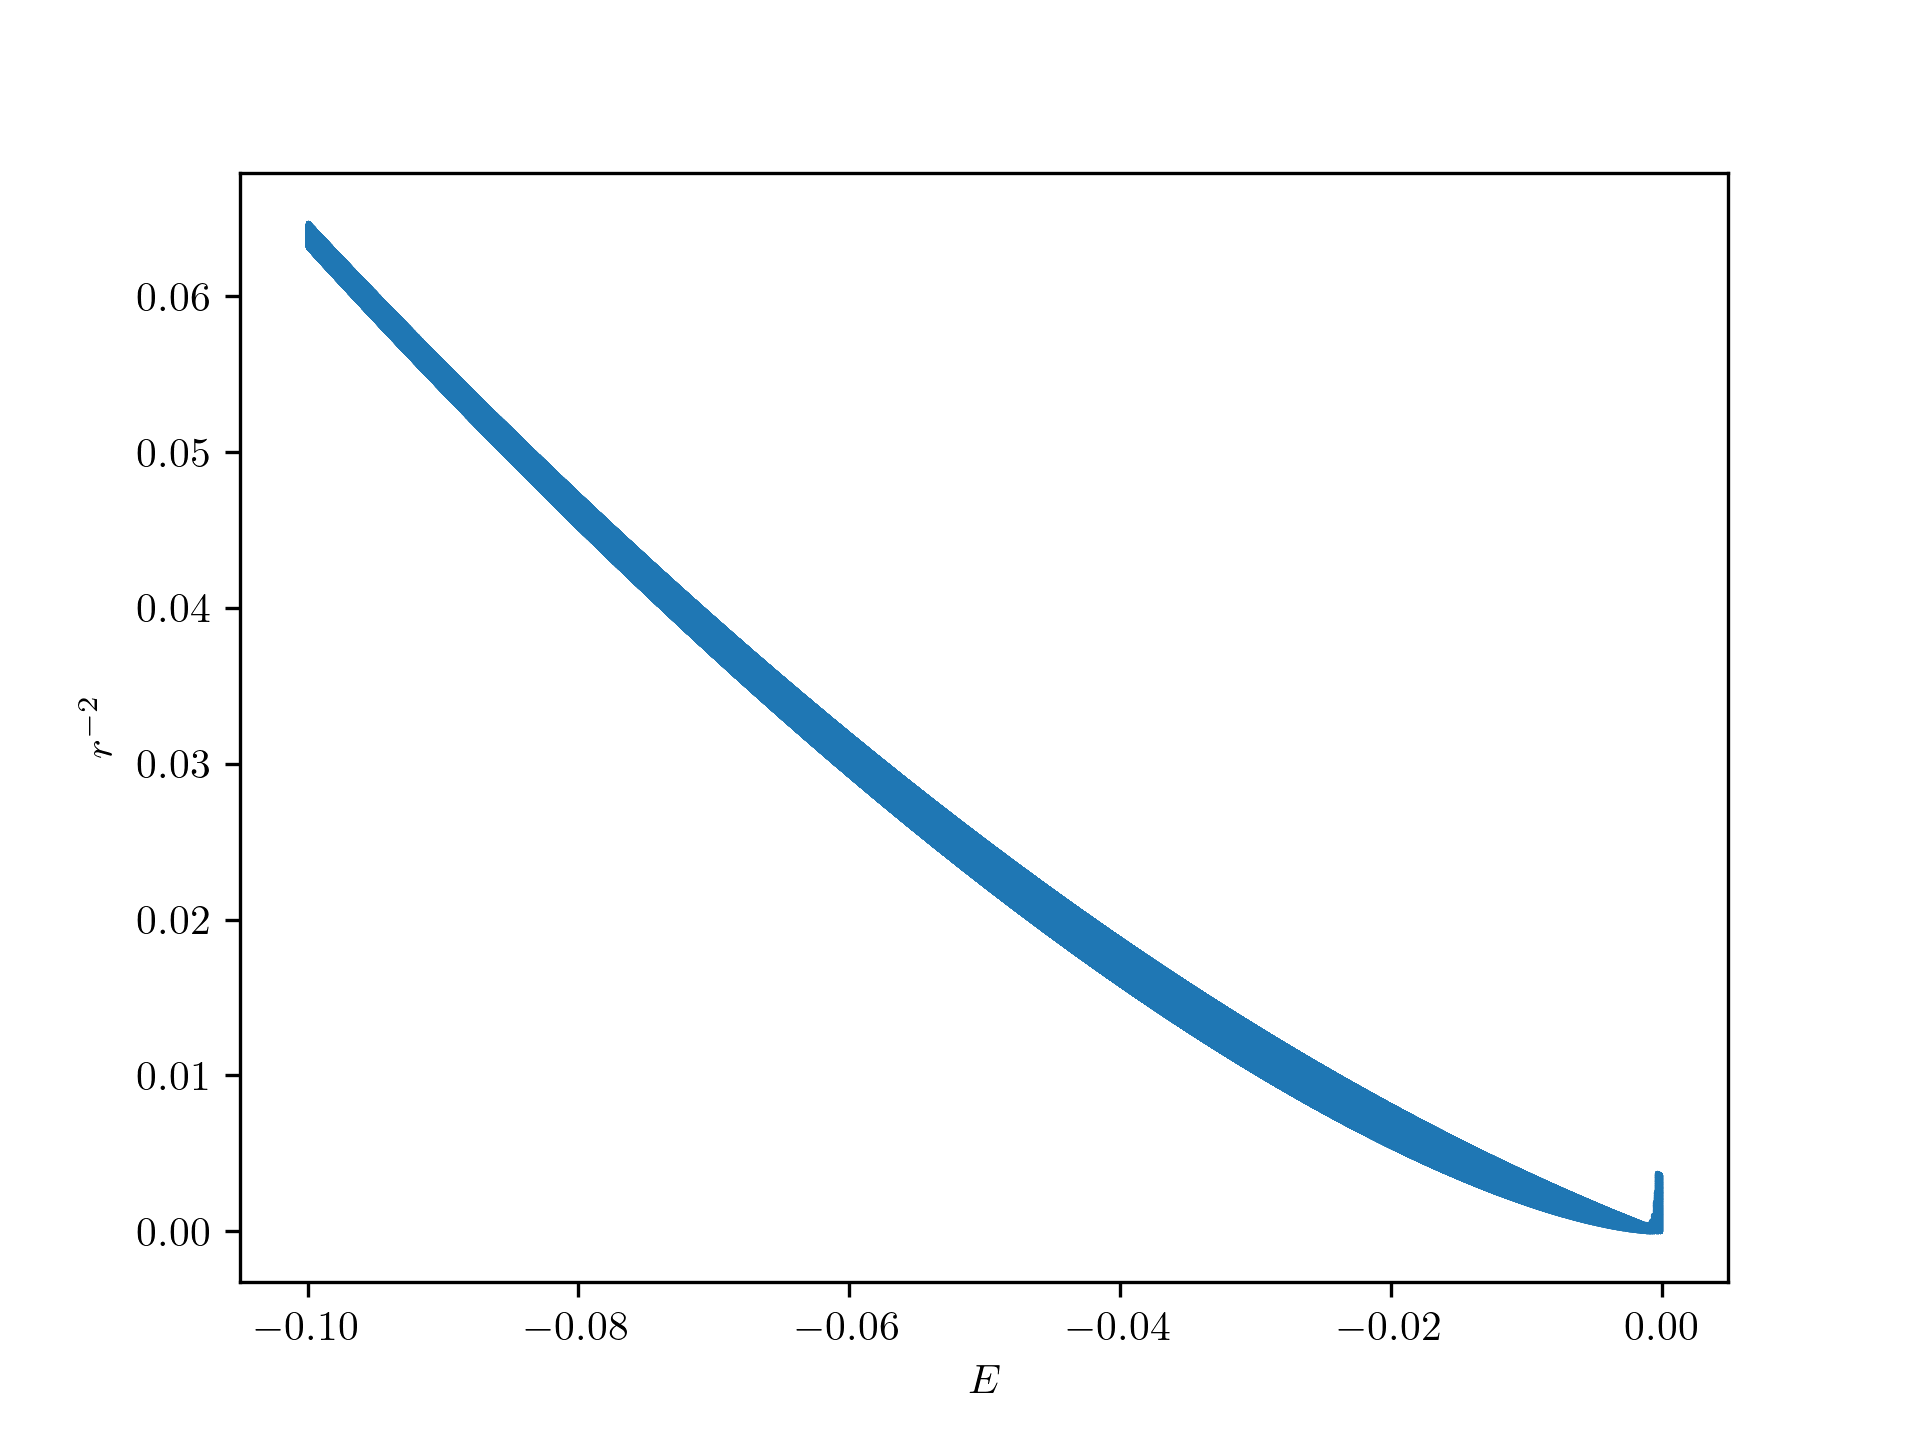
\includegraphics[width=0.8\linewidth]{noise.png}
		\caption{Noise around $E=0$ in coulomb potential}
	\end{figure}
	With the scale of matrix growing at a fourth power rate, the floating-point precision becomes a bottleneck of our program as $k$ grows. The typical \texttt{double} type in \texttt{c++} no longer meets our need since the range of the eigenvalues can easily exceed $10^{18}$ and thus leading to the loss of numerical precision in floating-point operations. In the coulomb potential above, this loss of precision will lead to some visible noise in the allowed region, resulting in a bulge where $E$ is around $0$. To eliminate this noise we set the precision in the code to 128 bits, as in Fig.\ref{fig:coulomb1}.

	The code is written in \texttt{c++} with the Eigen library~\cite{eigenweb} for linear algebra and GNU MPFR~\cite{fousse2007mpfr} for multiple precision floating-point.
	
% If you have acknowledgments, this puts in the proper section head.
%\begin{acknowledgments}
% put your acknowledgments here.
%\end{acknowledgments}

% Create the reference section using BibTeX:
\bibliography{main}

\end{document}
%
% ****** End of file apstemplate.tex ******
